\documentclass[11pt]{article}
\usepackage[top=1.00in, bottom=1.0in, left=1in, right=1in]{geometry}
\renewcommand{\baselinestretch}{1.1}
\usepackage{Sweave}
\usepackage{graphicx}
\usepackage{natbib}
\usepackage{amsmath}
\usepackage{gensymb}
\usepackage{parskip}
\usepackage{xcolor}
\usepackage{xr-hyper}
\usepackage{hyperref} 
\externaldocument{bayesianflows}

\def\labelitemi{--}

\usepackage{fancyhdr}
\pagestyle{fancy}
\fancyhead[LO]{}
\fancyhead[RO]{}

\begin{document}
\bibliographystyle{/Users/Lizzie/Documents/EndnoteRelated/Bibtex/styles/amnat}

\renewcommand{\refname}{\CHead{}}


\title{Supplement: A four-step simulation-based workflow for improving ecological science}
% \date{\today}
\author{EM Wolkovich, TJ Davies, WD Pearse \& M Betancourt}
\maketitle
\

\renewcommand{\thetable}{S\arabic{table}}
\renewcommand{\thefigure}{S\arabic{figure}}

\section*{Next steps}
Our aim is to provide an approachable succinct description of a basic adaptable workflow for those new to fitting complex models. Thus anyone wanting to implement it would likely benefit from more reading, training and/or community support. We highlight some resources in the main text, but more are being produced often and our suggestions are in no way intended to be comprehensive, so we recommend checking for additional resources. For those interested in this workflow and looking for somewhere to start, we suggest:
\begin{itemize}
\item A number of books and online resources provide approachable introductions to fitting Bayesian models that include a similar workflow to the one we outline here. These include: \emph{Statistical Rethinking} \citep{statrethink}, M. Betancourt's organized writing covering probability theory to modeling and inference \url{https://betanalpha.github.io/writing/}, \emph{Regression and Other Stories} \citep{regotherstories}. Many of these have related resources including additional examples, videos of courses taught using the materials and more (see, for example: \url{https://github.com/rmcelreath/stat_rethinking_2023} and \\ \url{https://avehtari.github.io/ROS-Examples/}). 
\item \citet{BDA} provides a comprehensive review of Bayesian inference, including many modeling approaches. 
\item A number of communities support learning these approaches, but tracking them down can take some inquiries depending on your specific interests and aims. We suggest attending conferences and visiting online support sites (e.g., \url{https://discourse.mc-stan.org/} or \url{https://www.r-inla.org/discussion-group}) and asking about how people connect. For example, ask about Slack or Discord servers or check for Meetup groups. 
\end{itemize}

\section*{A brief review of statistical inference using Bayesian approaches}

To fit bespoke models we usually apply Bayes' theorem, which generates a $posterior$ distribution from a combination of a $likelihood$ and a $prior$ distribution (an initial uncertainty estimate derived from basic ecological knowledge), and using iterative algorithms (e.g. MCMC, Markov Chain Monte Carlo) that provide samples that can be used to extract information from the posterior distribution (for more, see \emph{A brief review of statistical inference using Bayesian approaches} in the Supplement). 

% Robust analyses rely on our inferences being consistent with the underlying truth more often than not.  Quantifying this consistency is calibration---analyzing how often a parameter estimate is close to the true value---a critical part of using models for inference. A major problem with traditional (frequentist) approaches in ecology today is their inferences are unpredictable when their foundational assumptions are not met, but ecologists are not usually trained in how to recognize or deal with this.
% Most ecologists are trained primarily in frequentist methods, which are focused on calibration (this is is why training in frequentist methods includes so much discussion of significance, power, mean squared error, and the like). Bayesian methods typically focus on inference, but can be equally well calibrated (see Step 1, below). 

To better understand our workflow, we provide a very brief overview of some of the fundamentals of Bayesian methods that is inherently incomplete and, by design, not very technical. This section can be skipped for those who feel already well-versed, and can be augmented for those who are new to Bayesian approaches \citep[for example,][]{statrethink,BDA,regotherstories}.

Probability is often defined as ``the long-term frequency with which something happens.'' We would expect, for example that if we tossed a coin 100 times we would see roughly 50 heads. In this case we would say that the probability of tossing a coin and getting a `head' is $\frac{50}{100}$, equivalent to 50\% or $\frac{1}{2}$. At the same time we wouldn't be very surprised if we observed 49 or even 55 heads, although we would be surprised if we saw 99.

This definition of probability---which is the \emph{frequentist} definition---is useful in many situations, but it has a few disadvantages. First, frequentist probabilities are grounded in the assumption of repeated events. Using frequentist statistics requires trying to match a model that we have (often just in our heads) of some ecological system to a frequentist method that mostly closely matches the assumptions of our biological model. Second, this definition precludes the use of probability in quantifying inferences, so frequentist approaches are generally limited to point estimators and interval estimators.  The behavior of point estimators can be very sensitive to the model assumptions, and even small violations of the model assumptions can make the point estimator behavior difficult to quantify. Given the complexity of ecological data and our uncertainty about the underlying model, frequentist approaches can be especially challenging in ecology. 

Bayesian methods use probability more generally, allowing it to be used to quantify variation it the data but also uncertainty in our inferences about how ecological systems work. $Probability$ is used to quantify uncertainty: the higher the probability of a certain interval of values the less uncertainty we have that the true behavior falls within that interval. Assuming we also have some estimate of our initial uncertainty---usually from knowledge of ecology---to inform a prior distribution (termed below $prior$), then we can apply Bayes' theorem

\begin{equation}
  probability = \frac{likelihood \cdot prior}{normaliser}
  \label{bayes_theorem}
\end{equation}

to update that prior into a posterior distribution that accounts for the information added by a likelihood ($likelihood$ is the same as a frequentist likelihood). Here, \texttt{normaliser} is a mathematical constant that makes sure our probability cannot go above 100\% or below 0\%. This mathematical constant is a nuisance term that is extremely challenging to calculate (sometimes it is impossible!) and held back the practical use of Bayesian statistics for almost a century because that normaliser could rarely be analytically worked out. But one of the major advantages of Bayesian methods is that the solution to this problem---numerical simulations based on Markov Chain Monte Carlo (MCMC)---provide a huge additional advantage. Now that no analytical solution needs be found, any model that can be written out mathematically can be fit to data, giving the scientist more freedom of model structure.

% Nowadays, with increases in computer power, we can use numerical methods such as `Markov Chain Monte Carlo' (MCMC) methods to avoid having to estimate its value precisely. Such methods are iterative algorithms  that involve chance at each step (that the process proceeds in iterations or steps, and only the last iteration affects the next, is why this is a `Markov Chain'), tweaking and changing parameters within your model until a distribution of parameters consistent with the data are found. This distribution is called the `posterior' distribution to distinguish how it is our view of probability \emph{after} the data (via the likelihood) and the prior have been considered. %There is no guarantee that the posterior distribution will, itself, be found: the user must check for so-called `convergence' onto the true posterior distribution as the process involves randomness. It is for this randomness that `Monte Carlo' is added into the name, after a city famous for gambling.

% It turns out there is a further advantage that such an approach gives us. While frequentist probabilities are all about the probabilities of observing data ($p(data|model)$: what are the chances of getting 99 heads in 100 coin-tosses?), Bayesian probabilities are all about the probabilities of observing models ($p(model|data)$: what are the chances this coin is biased towards heads?). This makes it straightforward to report the results of Bayesian analyses in terms of estimates of uncertainty and precision of coefficients (contrast ``I'm 80\% certain that coin comes up heads at least two-thirds of the time'' with ``I'm less than 5\% certain those last twenty coin tosses came from a fair coin'').

\section*{Which workflow?}

Formally, all a `workflow' does is organize various steps together in a systematic fashion, but there are many different workflows depending on what the aim is, which will determine which steps a workflow should include. For example a workflow aimed at calibration could look like an expanded version of our Step 1, where all the steps focus on investigating the assumptions encoded in a given model using simulated data. Or a workflow aimed at inference could expand Step 3, to focus on constructing a posterior, then investigating its model adequacy via several criteria. An inferential workflow can also be extended into a model development workflow.  If the model adequacy criteria inform not only that something is inadequate about the current model assumptions but what is inadequate (ideally this happens some in Step 4) then one can use those hints to iterative improve the modeling assumptions. We present in the main text a very simplified model development workflow that combines calibration, inference and some model development, but it is not necessarily appropriate for everyone, depending on their aims.

% Ultimately it may be helpful to advocate for workflows, plural.  Bayesian methodologies can be used to systematically investigate the consequences of a given model, such as an estimator calibration workflow.  They can also be used to formalize heuristic residual checking with posterior retrodictive check and implement an iterative model development workflow.  Etc, etc.  The goal is to identify what you want to do and organize the steps to achieve that output as systematically as possible.


\section*{An example workflow}

Our workflow in the main text is explained mostly program-agnostically. Though at times we assume a user of \textsf{Stan}, a relatively new probabilistic programming language, that interfaces with \textsf{R, Python, Julia} (and more) to write bespoke Bayesian models \citep{Carpenter:2017stan}. We focus on \textsf{Stan} as its MCMC algorithm (a variant of Hamiltonian Monte Carlo, HMC) is fast and produces specific output to warn of model fit issues (i.e., divergent transitions) in a way other MCMC algorithms do not (e.g. Metropolis-Hastings or Gibbs), but the basic workflow should apply to diverse implementations of Bayesian modeling, and can be extended to other approaches (frequentist, resampling, etc.). 

% For our example workflow we use \textsf{Stan} and \textsf{R}, presented in Markdown (\verb|example.md| available at: \url{https://github.com/lizzieinvancouver/bayesianflowsexample}). 
For our example workflow we use \textsf{Stan} and \textsf{R}, presented in Markdown (see files). As our goal is to introduce people to this approach, we present a simple---but real-world---example to walk through the basic steps. Like all models, it is a work in progress, and could easily be adjusted, expanded and likely improved (all data and code will be fully and freely available on Zenodo before publication).
% For now, you can download the workflow here:
% \url{https://github.com/lizzieinvancouver/bayesianflows/blob/main/examples/synchrony/example.html}.

\section*{References}
\vspace{-5ex}
\bibliography{refs/bayesrefsmini.bib}


\section*{Figures}

\begin{figure}[ht]
\centering
\noindent 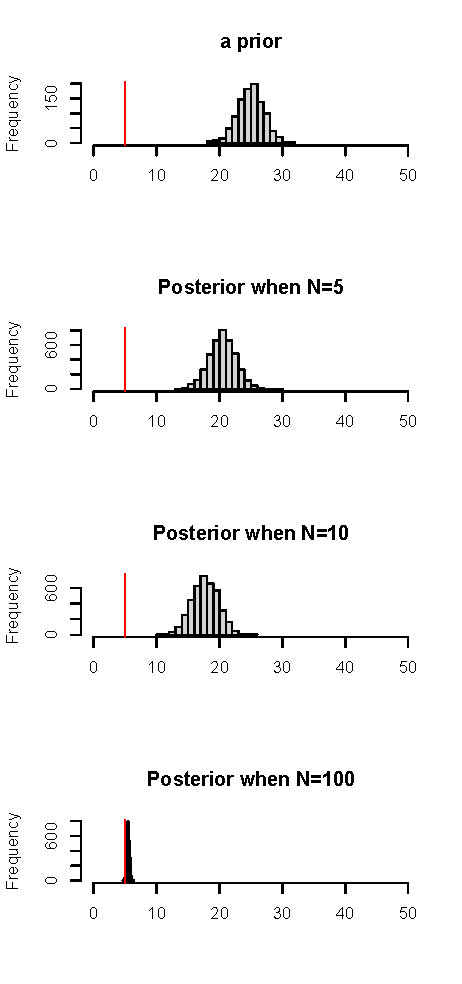
\includegraphics[width=0.5\textwidth]{examples/misspecifiedmodel/priorpostforflows.pdf}
\caption{A simple example of how to use simulated data to understand calibration issues in a mis-specified model. Here we know the true model underlying the data is $y=\alpha + \text{normal}(0, \sigma)$ where $\alpha$ is 5 (shown as blue vertical line) and $\sigma$ is 2. The model, however, is mis-specified by a prior for $\alpha$ of $\text{normal}(25, 2)$ (dashed blue line), resulting in a posterior (salmon-colored histogram) not centered on the true value. In our experience it is quite rare to have a prior informed by ecological knowledge be so far off, but this is an example. How mis-calibrated the model will be depends on the data: we show examples with a sample size ($N$) of 5, 10 and 40 data points. In practice these studies would allow us to determine how much data we would need to be robust to suspect prior models. }
\label{fig:misspecifyprior}
\end{figure}


\end{document}

\clearpage
\section{Figures}

\begin{figure}[ht]
\centering
\noindent 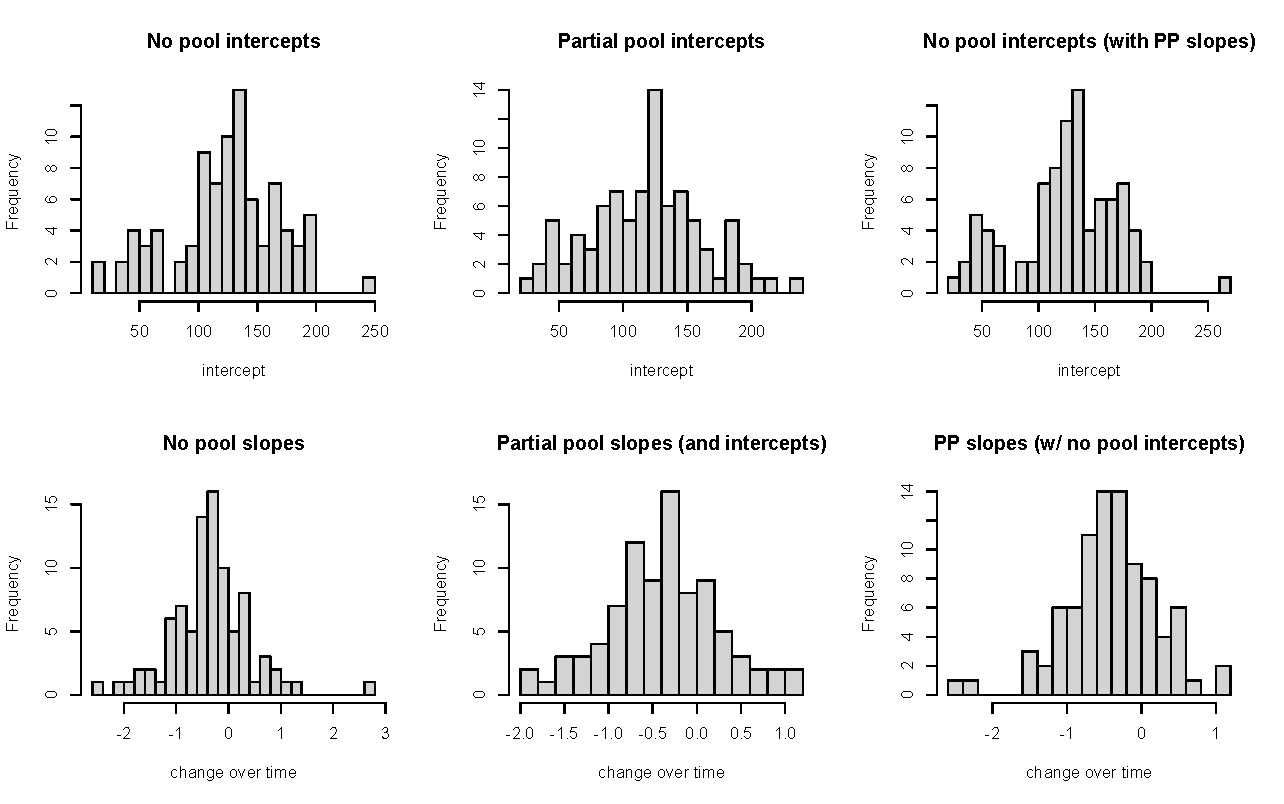
\includegraphics[width=1\textwidth]{examples/synchrony/graphs/compareppmodels.pdf}
\caption{Comparison of three types of models we fit: no pooling (right), partial pooling on slopes and intercept (middle) and partial pooling on slopes only (left).}
\label{fig:ppmodels}
\end{figure}

\section{Where to next?}

% Our workflow and its description is brisk, and thus anyone wanting to implement it would benefit from more reading. There are new good resources on this sort of workflow, and more being published often, but for now we especially recommend: 




I think that it would also be useful to mention residual analysis. Overall we need to compare model retrodictions to the observed data, projected onto the features relevant to the analysis. Classical residual analysis compares point predictions to the observe data. R2 summarizes this comparison as a linear correlation. Posterior retrodictive checks compare an entire distribution of predictions to the observed data, allowing us to not only identify any inconsistencies but also use the probabilistic spread of the predictions to qualify how important any inconsistencies are.

Feedbacks 

`Developing simulated data to test the model, running prior and retrodictive checks all dive you deep into understanding
your statistical model, which suddenly you may find yourself thinking through much more mechanistically.' I wonder if
it's beneficial to frame this more as `dive deep into connecting your statistical model to your domain expertise'?  I
often find myself trying to emphasize that people already have the domain expertise but they're not incorporating it into
their analyses.  A lot of what this workflow is trying to do is facilitate that integration to leverage what the analysts
have always had!
